\chapter{Topological Spaces and Continuous Functions}\label{chap:topological-spaces}
\section{Topologies}
\subsection{Definitions and Examples}
\begin{definition}[Topological space]
A collection $\mathcal{T}$ of subsets of a set $X$ is said to be a \vocab{topology}\index{topology} on $X$ if
\begin{enumerate}[label=(\roman*)]
\item $\emptyset,X\in\mathcal{T}$;
\item if $\{U_i\mid i\in I\}$ are in $\mathcal{T}$, then $\bigcup_{i\in I}U_i\in\mathcal{T}$;\hfill(closed under arbitrary unions)
\item if $U_1,\dots,U_n\in\mathcal{T}$, then $\bigcap_{i=1}^{n}U_i\in\mathcal{T}$.\hfill(closed under finite intersections)
\end{enumerate}
If $\mathcal{T}$ is a topology on $X$, then $(X,\mathcal{T})$ is a \vocab{topological space}\index{topological space}, and the members of $\mathcal{T}$ are called \emph{open sets} in $X$.
\end{definition}

\begin{notation}
If the topology $\mathcal{T}$ is clear, we simply omit it and denote a topological space as $X$.
\end{notation}

\begin{example}
Let $X$ be any non-empty set.
\begin{itemize}
\item The \emph{discrete topology} on $X$ is the set of all subsets of $X$; that is, $\mathcal{T}=\mathcal{P}(X)$.
\item The \emph{indiscrete topology} (or \emph{trivial topology}) on $X$ is $\mathcal{T}=\{X,\emptyset\}$.
\item The \emph{co-finite topology} on $X$ consists of the empty set together with every subset $U$ of $X$ such that $X\setminus U$ is finite.
\item Any metric space $(X,d)$, with $\mathcal{T}$ equal to the collection of all subsets of $X$ that are open in the metric space sense. This topology is called the \emph{metric topology} on $X$.
\end{itemize}
\end{example}

\begin{definition}
Suppose $\mathcal{T}$ and $\mathcal{T}^\prime$ are two topologies on a given set $X$. We say that
\begin{enumerate}[label=(\roman*)]
\item $\mathcal{T}$ is \vocab{finer}\index{finer} than $\mathcal{T}^\prime$ if $\mathcal{T}\supset\mathcal{T}^\prime$;
\item $\mathcal{T}$ is \vocab{coarser}\index{coarser} than $\mathcal{T}^\prime$ if $\mathcal{T}\subset\mathcal{T}^\prime$;
\item $\mathcal{T}$ is \vocab{comparable}\index{comparable} with $\mathcal{T}^\prime$ if either $\mathcal{T}\supset\mathcal{T}^\prime$ or $\mathcal{T}\subset\mathcal{T}^\prime$.
\end{enumerate}
\end{definition}

\begin{example}
The indiscrete topology is the coarsest topology possible, while the discrete topology is the finest topology possible.
\end{example}
\pagebreak

\subsection{Bases}
In linear algebra, every vector space is generated by a basis. In topology, we have a similar notion, as it is usually hard to define a topology by specifying all the open sets.

\begin{definition}[Basis]\label{defn:topology-basis}
A \vocab{basis}\index{basis} for a topology on $X$ is a collection $\mathcal{B}$ of subsets of $X$ (called \emph{basis elements}) if
\begin{enumerate}[label=(\roman*)]
\item for all $x\in X$, there exists $B\in\mathcal{B}$ such that $x\in B$;
\item for all $B_1,B_2\in\mathcal{B}$ and $x\in B_1\cap B_2$, there exists $B_3\in\mathcal{B}$ such that $x\in B_3\subset B_1\cap B_2$.
\end{enumerate}
\end{definition}

Property (i) states that the elements of $\mathcal{B}$ cover $X$. Property (ii) can be visualised as follows:

\begin{figure}[H]
\centering
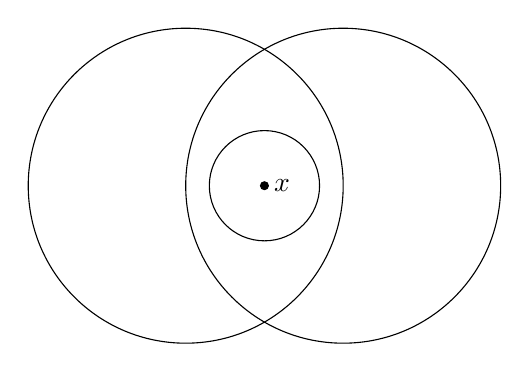
\begin{tikzpicture}
\draw[fill=black] (1.0,0.0) circle[radius=0.05cm] node [anchor=west] {$x$};
\draw (0.0,0.0) circle[radius=2.0cm];
\draw (2.0,0.0) circle[radius=2.0cm];
\draw (1.0,0.0) circle[radius=0.7cm];
\end{tikzpicture}
\caption{Property (ii) of \cref{defn:topology-basis}}
\end{figure}

\begin{definition}[Topology generated by basis]
We define the \emph{topology $\mathcal{T}$ generated by basis $\mathcal{B}$}\index{topology generated by basis} as follows:
\[U\in\mathcal{T}\iff\forall x\in U,\quad\exists B\in\mathcal{B},\quad x\in B\subset U.\]
\end{definition}

\begin{lemma*}
The collection $\mathcal{T}$ generated by the basis $\mathcal{B}$ is indeed a topology on $X$.
\end{lemma*}

\begin{proof} \
\begin{enumerate}[label=(\roman*)]
\item $\emptyset$ satisfies the defining condition of openness vacuously, so $\emptyset\in\mathcal{T}$. $X\in\mathcal{T}$ follows from (i) of \cref{defn:topology-basis}.

\item Let $\{U_i\mid i\in I\}$ be a collection of elements of $\mathcal{T}$. We want to show that $U=\bigcup_{i\in I}U_i\in\mathcal{T}$. 

Let $x\in U$. Then $x\in U_i$ for some $i\in I$. Since $U_i\in\mathcal{T}$, there exists $B\in\mathcal{B}$ such that $x\in B\subset U_i$. Thus $x\in B\subset U$, so $U\in\mathcal{T}$.

\item Let $U_1,U_2\in\mathcal{T}$. We want to show that $U_1\cap U_2\in\mathcal{T}$.

Let $x\in U_1\cap U_2$. Since $U_1\in\mathcal{T}$, there exists $B_1\in\mathcal{B}$ such that $x\in B_1\subset U_1$; since $U_2\in\mathcal{T}$, there exists $B_2\in\mathcal{B}$ such that $x\in B_2\subset U_2$. Then $x\in B_1\cap B_2$.

Since $\mathcal{B}$ is a basis, by (ii) of \cref{defn:topology-basis}, there exists $B_3\in\mathcal{B}$ such that $x\in B_3\subset B_1\cap B_2$. Thus $U_1\cap U_2\in\mathcal{T}$.

Finally, we show by induction that any finite intersection $U_1\cap\cdots\cap U_n\in\mathcal{T}$. This is trivial for $n=1$; suppose it true for $n-1$ and prove it
for $n$. Now
\[(U_1\cap\cdots\cap U_n)=(U_1\cap\cdots\cap U_{n-1})\cap U_n.\]
By hypothesis, $U_1\cap\cdots\cap U_{n-1}\in\mathcal{T}$. Thus the intersection of $U_1\cap\cdots\cap U_{n-1}$ and $U_n$ also belongs to $\mathcal{T}$.
\end{enumerate}
\end{proof}

Another way of describing the topology generated by a basis is given in the following result:

\begin{lemma}\label{lemma:topology-generated-basis-unions}
Let $\mathcal{T}$ be the topology on $X$ generated by basis $\mathcal{B}$. Then $\mathcal{T}$ equals the collection of all unions of elements of $\mathcal{B}$.
\end{lemma}

\begin{proof}
Let $\mathcal{B}=\{B_i\mid i\in I\}$.

\fbox{$\supset$} If $B_i\in\mathcal{B}$, see that
\[\forall x\in B_i,\quad x\in B_i\subset B_i\implies B_i\in\mathcal{T}.\]
Since $\mathcal{T}$ is a topology, the arbitrary unions of $B_i$'s must be in $\mathcal{T}$.

\fbox{$\subset$} Let $U\in\mathcal{T}$. Then for each $x\in U$, there exists $B_x\in\mathcal{B}$ such that $x\in B_x\subset U$. Then $U=\bigcup_{x\in U}B_x$, so $U$ is a union of elements of $\mathcal{B}$.
\end{proof}

\begin{remark}
The above result states that every $U\in\mathcal{T}$ can be expressed as a union of basis elements.
\end{remark}

We have described in two different ways how to go from a basis to the topology it generates. Sometimes we need to go in the reverse direction, from a topology to a basis generating it. Here is one useful way of obtaining a basis for a given topology.

\begin{lemma}\label{lemma:obtain-basis-for-given-topology}
Let $(X,\mathcal{T})$ be a topological space. Suppose that $\mathcal{C}$ is a collection of open sets of $X$, such that
\[\forall U\in\mathcal{T},\quad\forall x\in U,\quad\exists C\in\mathcal{C},\quad x\in C\subset U.\]
Then $\mathcal{C}$ is a basis for $\mathcal{T}$.
\end{lemma}

\begin{proof}
We first show that $\mathcal{C}$ is a basis.
\begin{enumerate}[label=(\roman*)]
\item For all $x\in X$, since $X\in\mathcal{T}$, by hypothesis, there exists $C\in\mathcal{C}$ such that $x\in C\subset X$.
\item Let $x\in C_1\cap C_2$, where $C_1,C_2\in\mathcal{C}\subset\mathcal{T}$. Thus $C_1,C_2\in\mathcal{T}$, so $C_1\cap C_2\in\mathcal{T}$. By hypothesis, there exists $C_3\in\mathcal{C}$ such that $x\in C_3\subset C_1\cap C_2$.
\end{enumerate}

Let $\mathcal{T}^\prime$ be the topology generated by $\mathcal{C}$; that is,
\[U\in\mathcal{T}^\prime\iff\forall x\in U,\quad\exists C\in\mathcal{C},\quad x\in C\subset U.\]
We will show that $\mathcal{T}=\mathcal{T}^\prime$.

\fbox{$\subset$} Let $U\in\mathcal{T}$, $x\in U$. By hypothesis, there exists $C\in\mathcal{C}$ such that $x\in C\subset U$. By definition, $U\in\mathcal{T}^\prime$. Hence $\mathcal{T}\subset\mathcal{T}^\prime$.

\fbox{$\supset$} Conversely, let $W\in\mathcal{T}^\prime$. By \ref{lemma:topology-generated-basis-unions}, $W$ is a union of elements of $\mathcal{C}$. Since each element of $\mathcal{C}$ is an element of $\mathcal{T}$ (and thus open), and a union of open sets is open, we have $W\in\mathcal{T}$. Hence $\mathcal{T}^\prime\subset\mathcal{T}$.
\end{proof}

When topologies are given by bases, the next result is a criterion to determine whether one topology is finer than another.

\begin{lemma}\label{lemma:topology-finer-criterion}
Let $\mathcal{B}$ and $\mathcal{B}^\prime$ be bases for the topologies $\mathcal{T}$ and $\mathcal{T}^\prime$ respectively on $X$. Then the following are equivalent:
\begin{enumerate}[label=(\roman*)]
\item $\mathcal{T}^\prime$ is finer than $\mathcal{T}$.
\item For all $x\in X$, and for all $B\in\mathcal{B}$ such that $x\in B$, there exists $B^\prime\in\mathcal{B}^\prime$ such that $x\in B^\prime\subset B$.
\end{enumerate}
\end{lemma}

\begin{figure}[H]
\centering
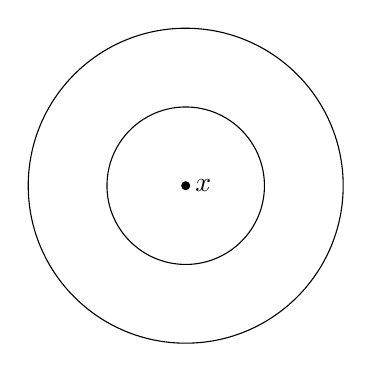
\begin{tikzpicture}
\draw[fill=black] (0.0,0.0) circle[radius=0.05cm] node [anchor=west] {$x$};
\draw (0.0,0.0) circle[radius=2.0cm];
\draw (0.0,0.0) circle[radius=1.0cm];
\end{tikzpicture}
\caption{(ii) of \ref{lemma:topology-finer-criterion}}
\end{figure}

\begin{proof} \

\fbox{(ii)$\implies$(i)} Let $U\in\mathcal{T}$. To show that $\mathcal{T}\subset\mathcal{T}^\prime$, we want to show that $U\in\mathcal{T}^\prime$.

Let $x\in U$. Since $\mathcal{B}$ generates $\mathcal{T}$, there exists $B\in\mathcal{B}$ such that $x\in B\subset U$. By (ii), there exists $B^\prime\in\mathcal{B}^\prime$ such that $x\in B^\prime\subset B$. Then $x\in B^\prime\subset U$, so $U\in\mathcal{T}^\prime$, by definition.

\fbox{(i)$\implies$(ii)} We are given $x\in X$ and $B\in\mathcal{B}$, with $x\in B$.

Now $B\in\mathcal{T}$ by definition, and $\mathcal{T}\subset\mathcal{T}^\prime$ by (i); therefore, $B\in\mathcal{T}^\prime$. Since $\mathcal{T}^\prime$ is generated by $\mathcal{B}^\prime$, there exists $B^\prime\in\mathcal{B}^\prime$ such that $x\in B^\prime\subset B$.
\end{proof}

We now define three topologies on the real line $\RR$, all of which are of interest.

\begin{definition} \
\begin{enumerate}[label=(\roman*)]
\item Let $\mathcal{B}$ be the collection of all open intervals in $\RR$. The topology generated by $\mathcal{B}$ is called the \vocab{standard topology}\index{standard topology} on $\RR$.

Whenever we consider $\RR$, we shall suppose it is given this topology unless stated otherwise. 

\item Let $\mathcal{B}^\prime$ be the collection of all half-open intervals of the form $[a,b)$. The topology generated by $\mathcal{B}^\prime$ is called the \vocab{lower limit topology}\index{lower limit topology} on $\RR$. 

When $\RR$ is given the lower limit topology, we denote it by $\RR_\ell$.

\item Let $K=\{\frac{1}{n}\mid n\in\ZZ^+\}$, and let $\mathcal{B}^{\prime\prime}$ be the collection of all open intervals $(a,b)$, along with all sets of the form $K\setminus(a,b)$. The topology generated by $B^{\prime\prime}$ is called the \vocab{$K$-topology}\index{$K$-topology} on $\RR$.

When $\RR$ is given this topology, we denote it by $\RR_K$.
\end{enumerate}
\end{definition}

It is easy to see that all three of these collections are bases; in each case, the intersection of two basis elements is either another basis element or is empty. The relation between these topologies is the following:

\begin{lemma}
The topologies of $\RR_\ell$ and $\RR_K$ are strictly finer than the standard topology on $\RR$, but are not comparable with one another.
\end{lemma}

\begin{proof}
Let $\mathcal{T}$, $\mathcal{T}^\prime$, and $\mathcal{T}^{\prime\prime}$ be the topologies of $\RR$, $\RR_\ell$, and $\RR_K$, respectively. 

Given a basis element $(a,b)$ for $\mathcal{T}$ and a point $x$ of $(a,b)$, the basis element $[x,b)$ for $\mathcal{T}^\prime$ contains $x$ and lies in $(a,b)$. On the other hand, given the basis element $[x,d)$ for $\mathcal{T}^\prime$, there is no open interval $(a,b)$ that contains $x$ and lies in $[x,d)$. Thus $\mathcal{T}\subset\mathcal{T}^\prime$, so $\mathcal{T}^\prime$ is strictly finer than $\mathcal{T}$.

A similar argument applies to $\RR_K$. Given a basis element $(a,b)$ for $\mathcal{T}$ and a point $x$ of $(a,b)$, this same interval is a basis element for $\mathcal{T}^{\prime\prime}$ that contains $x$. On the other hand, given the basis element $B=(-1,1)\setminus K$ for $\mathcal{T}^{\prime\prime}$ and the point $0$ of $B$, there is no open interval that contains $0$ and lies in $\mathcal{B}$.

We leave it to you to show that the topologies of $\RR_\ell$ and $\RR_K$ are not comparable.
\end{proof}

Since the topology generated by a basis $\mathcal{B}$ may be described as the collection of arbitrary unions of elements of $\mathcal{B}$ (by \ref{lemma:topology-generated-basis-unions}), what happens if we start with a given collection of sets and take finite intersections of them as well as arbitrary unions? 
This leads to the notion of a \emph{subbasis} for a topology.

\begin{definition}[Subbasis]
A \vocab{subbasis}\index{subbasis} $\mathcal{S}$ for a topology on $X$ is a collection of subsets of $X$ whose union equals $X$.
\end{definition}

\begin{definition}[Topology generated by subbasis]
The \emph{topology $\mathcal{T}$ generated by the subbasis}\index{topology generated by subbasis} $\mathcal{S}$ is defined as the collection of all unions of finite intersections of elements of $\mathcal{S}$:
\[U\in\mathcal{T}\iff U=\text{union of finite intersections in }\mathcal{S}.\]
\end{definition}

\begin{lemma*}
The collection $\mathcal{T}$ generated by the subbasis $\mathcal{S}$ is a topology.
\end{lemma*}

\begin{proof}
Consider the collection
\[\mathcal{B}=\{\text{all finite intersections of elements of }\mathcal{S}\}.\]
It suffices to show that $\mathcal{B}$ is a basis, for then by \ref{lemma:topology-generated-basis-unions}, the collection $\mathcal{T}$ of all unions of elements of $\mathcal{B}$ is a topology.
\begin{enumerate}[label=(\roman*)]
\item Let $x\in X$. Then $x$ belongs to an element of $\mathcal{S}$, and thus belongs to an element of $\mathcal{B}$.
\item Let
\[B_1=S_1\cap\cdots\cap S_m,\quad B_2=S_1^\prime\cap\cdots\cap S_n^\prime\]
be two elements of $\mathcal{B}$. Their intersection
\[B_1\cap B_2=(S_1\cap\cdots\cap S_m)\cap(S_1^\prime\cap\cdots\cap S_n^\prime)\]
is also a finite intersection of elements of $\mathcal{S}$, so it belongs to $\mathcal{B}$.
\end{enumerate}
\end{proof}
\pagebreak

\section{Examples of Topologies}
\subsection{Order Topology}
\begin{definition}[Order topology]
Let $(X,<)$, $|X|>1$. Let $\mathcal{B}$ be the collection of all sets of the following types:
\begin{enumerate}[label=(\roman*)]
\item All open intervals $(a,b)$ in $X$.
\item All intervals of the form $[a_0,b)$, where $a_0$ is the smallest element (if any) of $X$.
\item All intervals of the form $(a,b_0]$, where $b_0$ is the largest element (if any) of $X$.
\end{enumerate}
The topology generated by $\mathcal{B}$ is called the \vocab{order topology}.
\end{definition}

We need to check that $\mathcal{B}$ is a basis of $X$.
\begin{enumerate}[label=(\roman*)]
\item Every $x\in X$ lies in some element of $\mathcal{B}$: the smallest element (if any) lies in all sets of type (ii), the largest element (if any) lies in all sets of type (iii), and every other element lies in a set of type (i).
\item The intersection of any two sets of the preceding types is a set of one of these types, or is empty. Several cases need to be checked; we leave it to you.

For instance, let $x\in(a,b)\cap(c,d)$. Let $p=\max\{a,c\}$, $q=\min\{b,d\}$. Then $x\in(p,q)\subset(a,b)\cap(c,d)$, where $(p,q)\in\mathcal{B}$.
\end{enumerate}

\begin{example}\hfill
\begin{itemize}
\item The standard topology on $\RR$ is just the order topology derived from the usual order on $\RR$.
\end{itemize}
\end{example}

\begin{definition}
Let $(X,<)$, $a\in X$. Then the following subsets of $X$ are \vocab{rays} determined by $a$:
\begin{align*}
(a,+\infty)&=\{x\in X\mid x>a\},\\
[a,+\infty)&=\{x\in X\mid x\ge a\},\\
(-\infty,a)&=\{x\in X\mid x<a\},\\
(-\infty,a]&=\{x\in X\mid x\le a\}.
\end{align*}
\end{definition}

$(a,+\infty)$ and $(-\infty,a)$ are called \emph{open rays}, since they are open; for instance, $(a,+\infty)=\bigcup_{x>a}(a,x)$. Similarly, $[a,+\infty)$ and $(-\infty,a]$ are \emph{closed rays}.

\begin{lemma}
The collection of open rays form a subbasis for the order topology.
\end{lemma}

\begin{proof}
Let $\mathcal{T}$ be the order topology on $X$, let $\mathcal{T}^\prime$ be the topology generated by the subbasis of open rays. We will show that $\mathcal{T}=\mathcal{T}^\prime$.
\begin{itemize}
\item Because the open rays are open in the order topology, the topology they generate is contained in the order topology. Hence $\mathcal{T}^\prime\subset\mathcal{T}$.
\item On the other hand, every basis element for the order topology equals a finite intersection of open rays; the interval $(a,b)$ equals the intersection of $(-\infty,b)$ and $(a,+\infty)$, while $[a_0,b)$ and $(a,b_0]$, if they exist, are themselves open rays. Hence the topology generated by the open rays contains the order topology, so $\mathcal{T}\subset\mathcal{T}^\prime$.
\end{itemize}
\end{proof}

\subsection{Product Topology}
If $X$ and $Y$ are topological spaces, there is a standard way of defining a topology on the cartesian product $X\times Y$. We consider this topology now and study some of its properties.

\begin{definition}[Product topology]
Let $(X,\mathcal{T}_X)$ and $(Y,\mathcal{T}_Y)$ be topological spaces. The \vocab{product topology}\index{product topology} on $X\times Y$ is the topology $\mathcal{T}_{X\times Y}$ with basis
\[\mathcal{B}=\{U\times V\mid U\in\mathcal{T}_X,V\in\mathcal{T}_Y\}.\]
\end{definition}

\begin{lemma*}
$\mathcal{B}$ is a basis.
\end{lemma*}

\begin{proof} \
\begin{enumerate}[label=(\roman*)]
\item $X\times Y$ is a basis element, so every element of $X\times Y$ is contained in $X\times Y$.
\item Let $U_1\times V_1,U_2\times V_2\in\mathcal{B}$. Then their intersection is
\[(U_1\times V_1)\cap(U_2\times V_2)=(U_1\cap U_2)\times(V_1\cap V_2).\]
Since $U_1\cap U_2\in\mathcal{T}_X$, $V_1\cap V_2\in\mathcal{T}_Y$, we have that $(U_1\cap U_2)\times(V_1\cap V_2)\in\mathcal{B}$.
\end{enumerate}
\end{proof}

What can one say if the topologies on $X$ and $Y$ are given by bases? The answer is as follows:

\begin{lemma}
If $\mathcal{B}$ is a basis for the topology of $X$, $\mathcal{C}$ is a basis for the topology of $Y$, then the collection
\[\mathcal{D}=\{B\times C\mid B\in\mathcal{B}, C\in\mathcal{C}\}\]
is a basis for the topology of $X\times Y$.
\end{lemma}

\begin{proof}
We apply \ref{lemma:obtain-basis-for-given-topology}.

Let $W$ be an open set of $X\times Y$, and let $(x,y)\in W$. By definition of product topology there exists a basis element $U\times V$ such that $(x,y)\in U\times V\subset W$. 

Since $\mathcal{B}$ and $\mathcal{C}$ are bases for $X$ and $Y$ respectively, there exists $B\in\mathcal{B}$ such that $x\in B\subset U$, and $C\in\mathcal{C}$ such that $y\in C\subset V$. Then $(x,y)\in B\times C\subset W$. 

Thus the collection $\mathcal{D}$ meets the criterion of \ref{lemma:obtain-basis-for-given-topology}, so $\mathcal{D}$ is a basis for $X\times Y$.
\end{proof}

\begin{definition}[Projection map]
Define the projection map of $X\times Y$ onto $X$ as
\begin{align*}
\pi_1\colon X\times Y&\to X\\
(x,y)&\mapsto x
\end{align*}
and the projection map of $X\times Y$ onto $Y$ as
\begin{align*}
\pi_2\colon X\times Y&\to Y\\
(x,y)&\mapsto y
\end{align*}
\end{definition}

\begin{remark}
We use the word ``onto'' because $\pi_1$ and $\pi_2$ are surjective (unless one of the spaces $X$ or $Y$ happens to be empty, in which case $X\times Y$ is empty and our whole discussion is empty as well!).
\end{remark}

If $U$ is an open subset of $X$, then the set $\pi_1^{-1}(U)$ is precisely the set $U\times Y$, which is open in $X\times Y$.
Similarly, if $V$ is open in $Y$, then $\pi_2^{-1}(V)=X\times V$, which is open in $X\times Y$.

\begin{lemma}
The collection
\[\mathcal{S}=\{\pi_1^{-1}(U)\mid U\text{ open in }X\}\cup\{\pi_2^{-1}(V)\mid V\text{ open in }Y\}\]
is a subbasis for the product topology on $X\times Y$.
\end{lemma}

\begin{proof}
Let $\mathcal{T}$ denote the product topology on $X\times Y$; let $\mathcal{T}^\prime$ be the topology generated by $\mathcal{S}$. We will show that $\mathcal{T}=\mathcal{T}^\prime$.

\fbox{$\supset$} Since every element of $\mathcal{S}$ belongs to $\mathcal{T}$, so do arbitrary unions of finite intersections of elements of $\mathcal{S}$. Thus $\mathcal{T}^\prime\subset\mathcal{T}$.

\fbox{$\subset$} Every basis element $U\times V$ for the topology $\mathcal{T}$ is a finite intersection of elements of $\mathcal{S}$, since
\[U\times V=\pi_1^{-1}(U)\cap\pi_2^{-1}(V).\]
Thus $U\times V$ belongs to $\mathcal{T}^\prime$, so $\mathcal{T}\subset\mathcal{T}^\prime$.
\end{proof}

\subsection{Subspace Topology}
\begin{definition}[Subspace topology]
Let $(X,\mathcal{T})$ be a topological space. If $Y\subset X$, the collection
\[\mathcal{T}_Y\colonequals\{Y\cap U\mid U\in\mathcal{T}\}\]
is a topology on $Y$, called the \vocab{subspace topology}\index{subspace topology}. With this topology, $Y$ is called a \vocab{subspace} of $X$; its open sets consist of all intersections of open sets of $X$ with $Y$.
\end{definition}

\begin{lemma*}
$\mathcal{T}_Y$ is a topology.
\end{lemma*}

\begin{proof} \
\begin{enumerate}[label=(\roman*)]
\item $\emptyset=Y\cap\emptyset$ so $\emptyset\in\mathcal{T}_Y$. $Y=Y\cap X$ so $Y\in\mathcal{T}_Y$.
\item $\mathcal{T}_Y$ is closed under finite intersections, since
\[(U_1\cap Y)\cap\cdots\cap(U_n\cap Y)=(U_1\cap\cdots\cap U_n)\cap Y.\]
\item $\mathcal{T}_Y$ is closed under arbitrary unions, since
\[\bigcup_{i\in I}(U_i\cap Y)=\brac{\bigcup_{i\in I}U_i}\cap Y.\]
\end{enumerate}
\end{proof}

\begin{lemma}
If $\mathcal{B}$ is a basis for the topology of $X$, then
\[\mathcal{B}_Y=\{B\cap Y\mid B\in\mathcal{B}\}\]
is a basis for the subspace topology on $Y$.
\end{lemma}

\begin{proof}
Let $U$ be open in $X$, $y\in U\cap Y$.
Since $\mathcal{B}$ is a basis for the topology of $X$, there exists $B\in\mathcal{B}$ such that $y\in B\subset U$. 
Then $y\in B\cap Y\subset U\cap Y$. 

By \ref{lemma:obtain-basis-for-given-topology}, $\mathcal{B}_Y$ is a basis for the subspace topology on $Y$.
\end{proof}

When dealing with a space $X$ and a subspace $Y$, one needs to be careful when one uses the term ``open set''. Does one mean an element of the topology of $Y$ or an
element of the topology of $X$? 

We make the following definition: If $Y$ is a subspace of $X$, we say that a set $U$ is \emph{open in} $Y$ if it belongs to the topology of $Y$; this implies in particular that it is a subset of $Y$. 
We say that $U$ is \emph{open in} $X$ if it belongs to the topology of $X$.

There is a special situation in which every set open in $Y$ is also open in $X$:

\begin{lemma}
Let $Y$ be a subspace of $X$. If $U$ is open in $Y$, and $Y$ is open in $X$, then $U$ is open in $X$.
\end{lemma}

\begin{proof}
Since $U$ is open in $Y$, $U=Y\cap V$ for some set $V$ open in $X$. Since $Y$ and $V$ are both open in $X$, so is $Y\cap V$.
\end{proof}

Now let us explore the relation between the subspace topology and the product topology.

\begin{lemma}
If $A$ is a subspace of $X$, and $B$ is a subspace of $Y$, then the product topology on $A\times B$ is the same as the topology $A\times B$ inherits as a subspace of $X\times Y$.
\end{lemma}

\begin{proof}
The set $U\times V$ is the general basis element for $X\times Y$, where $U$ is open in $X$ and $V$ is open in $Y$. 
Hence $(U\times V)\cap(A\times B)$ is the general basis element for the subspace topology on $A\times B$. 
Now
\[(U\times V)\cap(A\times B)=(U\cap A)\times(V\cap B).\]

Since $U\cap A$ and $V\cap B$ are the general open sets for the subspace topologies on $A$ and $B$, respectively, the set $(U\cap A)\times(V\cap B)$ is the general basis element for the product topology on $A\times B$.

The conclusion we draw is that the bases for the subspace topology on $A\times B$ and for the product topology on $A\times B$ are the same. Hence the topologies are the same.
\end{proof}
\pagebreak

\section{Closed Sets and Limit Points}
Let $X$ be a topological space.
If $E$ is an open set containing $x$, we say $E$ is a \vocab{neighbourhood} of $x$.

\subsection{Closed Sets}
\begin{definition}[Closed set]
We say $E\subset X$ is \vocab{closed}\index{closed set} if its complement $E^c=X\setminus E$ is open.
\end{definition}

The collection of closed subsets of a space $X$ has properties similar to those satisfied by the collection of open subsets of $X$:
\begin{lemma}
Let $X$ be a topological space.
\begin{enumerate}[label=(\roman*)]
\item $\emptyset$ and $X$ are closed.
\item Arbitrary intersections of closed sets are closed.
\item Finite unions of closed sets are closed.
\end{enumerate}
\end{lemma}

\begin{proof} \
\begin{enumerate}[label=(\roman*)]
\item $\emptyset$ and $X$ are closed because they are the complements of the open sets $X$ and $\emptyset$, respectively.
\item Suppose $\{A_i\mid i\in I\}$ is a collection of closed sets. By de Morgan's laws,
\[\brac{\bigcap_{i\in I}A_i}^c=\bigcup_{i\in I}{A_i}^c.\]
Since each ${A_i}^c$ is open, the RHS is open since it is an arbitrary union of open sets. Hence $\bigcap A_i$ is closed.
\item Suppose $A_i$ is closed for $i=1,\dots,n$. Then
\[\brac{\bigcup_{i=1}^{n}A_i}^c=\bigcap_{i=1}^{n}{A_i}^c.\]
The RHS is a finite intersection of open sets and is thus open. Hence $\bigcup A_i$ is closed.
\end{enumerate}
\end{proof}

\begin{remark}
Note that $\emptyset$ and $X$ are both open and closed. This explains the statement ``a door is not a set'': a door must be either open or closed, and cannot be both, while a set can be open, or closed, or both, or neither!
\end{remark}

\begin{remark}
Instead of using open sets, one could just as well specify a topology on a space by giving a collection of sets (to be called ``closed sets'') satisfying the three properties above. 
However this procedure has no particular advantage over the one we have adopted, so we shall use open sets to define topologies.
\end{remark}

If $Y$ is a subspace of $X$, we say $E$ is \emph{closed in} $Y$ if $E\subset Y$ and $E$ is closed in the subspace topology of $Y$ (that is, $Y\setminus E$ is open in $Y$).

\begin{proposition}
Let $Y$ be a subspace of $X$. Then $E$ is closed in $Y$ if and only if it equals the intersection of a closed set of $X$ with $Y$.
\end{proposition}

\begin{proof} \

\fbox{$\impliedby$} Suppose $E=C\cap Y$, where $C$ is closed in $X$.

Then $X\setminus C$ is open in $X$, so that $(X\setminus C)\cap Y$ is open in $Y$, by definition of subspace topology.

But $(X\setminus C)\cap Y=Y\setminus E$. Hence $Y\setminus E$ is open in $Y$, so that $E$ is closed in $Y$.

\fbox{$\implies$} Suppose $E$ is closed in $Y$. Then $Y\setminus E$ is open in $Y$.

By definition of subspace topology, $Y\setminus E$ is the intersection of an open set $U$ of $X$ with $Y$. Note that $X\setminus U$ is closed in $X$, and $E=Y\cap(X\setminus U)$. 
Thus $E$ equals the intersection of a closed set of $X$ with $Y$, as desired.
\end{proof}

A set $E$ that is closed in the subspace $Y$ may or may not be closed in the larger space $X$. As was the case with open sets, there is a criterion for $E$ to be closed in $E$:

\begin{proposition}
Let $Y$ be a subspace of $X$. If $E$ is closed in $Y$, and $Y$ is closed in $X$, then $E$ is closed in $X$.
\end{proposition}

\begin{proof}

\end{proof}
\pagebreak

\subsection{Closure and Interior}
\begin{definition}
The \vocab{interior}\index{interior} $\Int E$ of $E\subset X$ is the union of all open sets contained in $E$.

The \vocab{closure}\index{closure} $\overline{E}$ of $E$ is the intersection of all closed sets containing $E$.
\end{definition}

Obviously $\Int E$ is an open set and $\overline{E}$ is a closed set; furthermore,
\[\Int E\subset E\subset\overline{E}.\]
If $E$ is open, $E=\Int E$; while if $E$ is closed, $E=\overline{E}$.

We shall not make much use of the interior of a set, but the closure of a set will be quite important.

When dealing with a topological space $X$ and a subspace $Y$, one needs to exercise care in taking closures of sets. If $E$ is a subset of $Y$, the closure of $E$ in $Y$ and the closure of $E$ in $X$ will in general be different. 

\begin{notation}
We reserve the notation $\overline{E}$ to mean the closure of $E$ in $X$.
\end{notation}

The next result shows that the closure of $E$ in $Y$ can be expressed in terms of $\overline{E}$.

\begin{proposition}
Let $Y$ be a subspace of $X$; let $E\subset Y$, let $\overline{E}$ denote the closure of $E$ in $X$. Then the closure of $E$ in $Y$ equals $\overline{E}\cap Y$.
\end{proposition}

\begin{proof}
Let $F$ denote the closure of $E$ in $Y$. 
We will show that $F=\overline{E}\cap Y$.

\fbox{$\subset$} $\overline{E}$ is closed in $X$, so $\overline{E}\cap Y$ is closed in $Y$. 

Since $\overline{E}\cap Y$ contains $E$, and since by definition $F$ equals the intersection of all closed subsets of $Y$ containing $E$, we must have $F\subset(\overline{E}\cap Y)$.

\fbox{$\supset$} Since $F$ is closed in $Y$, $F=C\cap Y$ for some set $C$ closed in $X$. Then $C$ is a closed set of $X$ containing $E$; since $\overline{E}$ is the intersection of all such closed sets, we have $\overline{E}\subset C$. Then $(\overline{E}\cap Y)\subset(C\cap Y)=F$.
\end{proof}

The next result provides a convenient characterisation of the closure of a set.

\begin{lemma}\label{lemma:closure-characterisation}
If $E\subset X$, then $x\in\overline{E}$ if and only if every neighbourhood of $x$ intersects $E$.
\end{lemma}

\begin{proof} \

\forward We prove the contrapositive. Suppose $x\notin\overline{E}$.

Then $\overline{E}^c$ is an open set containing $x$ which does not intersect $E$, as desired.

\backward We prove the contrapositive. Suppose there exists a neighbourhood $U$ of $x$ which does not intersect $E$. 
Then $U^c$ is a closed set containing $E$. By definition of closure $\overline{E}$, $U^c$ must contain $\overline{E}$; hence $x$ cannot be in $\overline{E}$.
\end{proof}

\begin{corollary}
Supposing the topology of $X$ is given by a basis, then $x\in\overline{E}$ if and only if every basis element $B$ containing $x$ intersects $E$.
\end{corollary}

\begin{proof} \

\forward If every open set containing $x$ intersects $E$, so does every basis element $B$ containing $x$, because $B$ is an open set. 

\backward If every basis element containing $x$ intersects $E$, so does every open set $U$ containing $x$, because $U$ contains a basis element that contains $x$.
\end{proof}
\pagebreak

\subsection{Limit Points}
\begin{definition}
Suppose $E\subset X$. We say $x\in X$ is a \vocab{limit point}\index{limit point} of $E$, if every neighbourhood of $x$ intersects $E$ in some point other than $x$ itself.
\end{definition}

Let $E^\prime$ denote the set of all limit points of $E$.

We shall now see that limit points provide another way to describe the closure of a set.

\begin{proposition}
Let $E\subset X$. Then $\overline{E}=E\cup E^\prime$.
\end{proposition}

\begin{proof} \

\fbox{$\supset$} Let $x\in E^\prime$. Then every neighbourhood of $x$ intersects $E$ (in a point different from $x$).

By \ref{lemma:closure-characterisation}, $x\in\overline{E}$. Hence $E^\prime\subset\overline{E}$. Since $E\subset\overline{E}$, it follows that $E\cup E^\prime\subset\overline{E}$.

\fbox{$\subset$} Let $x\in\overline{E}$. 
\begin{itemize}
\item If $x\in E$, it is trivial that $x\in E\cup E^\prime$. 

\item If $x\notin E$, since $x\in\overline{E}$, we know that every neighbourhood $U$ of $x$ intersects $A$. Since $x\notin E$, the set $U$ must intersect $E$ in a point different from $x$. Then $x\in E^\prime$.
\end{itemize}
Thus $x\in E\cup E^\prime$, so $\overline{E}\subset E\cup E^\prime$.
\end{proof}

\begin{corollary}
$E\subset X$ is closed if and only if it contains all its limit points.
\end{corollary}

\begin{proof}
$E$ is closed if and only if $E=\overline{E}$, and the latter holds if and only if $E^\prime\subset E$.
\end{proof}
\pagebreak

\subsection{Hausdorff Spaces}
\begin{definition}[Hausdorff space]
A topological space $X$ is a \vocab{Hausdorff space}\index{Hausdorff space} if, for all distinct $x,y\in X$, there exist neighbourhoods $U$ and $V$ of $x$ and $y$ respectively that are disjoint.
\end{definition}

\begin{lemma}
Every finite point set in a Hausdorff space $X$ is closed.
\end{lemma}

\begin{proof}
It suffices to show that every one-point set $\{x_0\}$ is closed. 

If $x$ is a point of $X$ different from $x_0$, then $x$ and $x_0$ have disjoint neighbourhoods $U$ and $V$, respectively.
Since $U$ does not intersect $\{x_0\}$, the point $x$ cannot belong to the closure of the set $\{x_0\}$.

Hence the closure of $\{x_0\}$ is $\{x_0\}$ itself, so $\{x_0\}$ is closed.
\end{proof}

The condition that finite point sets be closed is in fact weaker than the Hausdorff condition. For example, $\RR$ in the finite complement topology is not a Hausdorff space, but it is a space in which finite point sets are closed. 

The condition that finite point sets be closed is called the \vocab{$T_1$ axiom}.

\begin{proposition}
Let $X$ be a space satisfying the $T_1$ axiom; let $E\subset X$. Then $x$ is a limit point of $E$ if and only if every neighbourhood of $x$ contains infinitely many points of $E$.
\end{proposition}

\begin{proof} \

\backward If every neighbourhood of $x$ intersects $E$ in infinitely many points, it certainly intersects $E$ in some point other than $x$ itself, so that $x$ is a limit point of $E$.

\forward Let $x$ be a limit point of $E$. Suppose, for a contradiction, that there exists a neighbourhood $U$ of $x$ which intersects $E$ at finitely many points.

Then $U$ also intersects $E\setminus\{x\}$ at finitely many points, say $x_1,\dots,x_m$; that is,
\[U\cap(E\setminus\{x\})=\{x_1,\dots,x_m\}.\]
Since the finite point set $\{x_1,\dots,x_m\}$ is closed, its complement $\{x_1,\dots,x_m\}^c$ is open. Then
\[U\cap\{x_1,\dots,x_m\}^c\]
is a neighbourhood of $x$ that does not intersect $E\setminus\{x\}$. This contradicts the assumption that $x$ is a limit point of $E$.
\end{proof}

\begin{definition}[Limit]
If a sequence $(x_n)$ in a Hausdorff space $X$ converges to $x\in X$, we write $x_n\to x$, and say $x$ is the \vocab{limit} of $(x_n)$.
\end{definition}

\begin{lemma}[Uniqueness of limit]
If $X$ is a Hausdorff space, then a sequence of points of $X$ converges to at most one point of $X$.
\end{lemma}

\begin{proof}
Suppose $(x_n)$ is a sequence in $X$, $x_n\to x$. 

If $y\neq x$, let $U$ and $V$ be disjoint neighborhoods of $x$ and $y$, respectively. Since $U$ contains $x_n$ for all but finitely many values of $n$, the set $V$ cannot. Therefore, $x_n\not\to y$.
\end{proof}

\begin{proposition}
Every simply ordered set is a Hausdorff space in the order topology. The product of two Hausdorff spaces is a Hausdorff space. A subspace of a Hausdorff space is a Hausdorff space.
\end{proposition}
\pagebreak

\subsection{Compactness}
\begin{definition}
We say $K\subset X$ is \vocab{compact} if every open cover of $K$ contains a finite subcover; that is, if $\{U_i\mid i\in I\}$ is a collection of open sets whose union contains $K$, then the union of some finite subcollection of $\{U_i\}$ also contains $K$.

In particular, if $X$ is itself compact, then $X$ is called a \emph{compact space}. 

$X$ is \emph{locally compact} if every point of $X$ has a neighbourhood whose closure is compact.
\end{definition}

Obviously, every compact space is locally compact.

We recall the Heine-Borel theorem: The compact subsets of a euclidean space $\RR^n$ are precisely those that are closed and bounded. From this it follows easily that $\RR^n$ is a locally compact Hausdorff space. Also, every metric space is a Hausdorff space.

The next result states that a closed subset of a compact set is compact.

\begin{lemma}
Suppose $K$ is compact and $F$ is closed, in a topological space $X$. If $F\subset K$, then $F$ is compact.
\end{lemma}

\begin{proof}
If $\{U_i\mid i\in I\}$ is an open cover of $F$ and $W=F^c$, then $W\cup\bigcup_{i\in I}U_i$ covers $X$; hence there is a finite collection $\{U_{i_k}\}$ such that
\[K\subset\bigcup_{k=1}^{n}U_{i_k}.\]
Then $F\subset\bigcup_{k=1}^{n}U_{i_k}$.
\end{proof}

\begin{corollary}
Suppose $A\subset B$. If $\overline{B}$ is compact, then $\overline{A}$ is compact.
\end{corollary}

\begin{proposition}
Suppose $X$ is a Hausdorff space, $K\subset X$ is compact, and $x\in K^c$. 
Then there exist open sets $U$ and $W$ such that $x\in U$, $K\subset W$, and $U\cap W=\emptyset$.
\end{proposition}

\begin{proof}
Let $y\in K$. The Hausdorff separation axiom implies the existence of disjoint open sets $U_y$ and $V_y$ such that $x\in U_y$ and $y\in U_y$. 
Since $K$ is compact, there exist points $y_1,\dots,y_n\in K$ such that
\[K\subset V_{y_1}\cup\cdots\cup V_{y_n}.\]
Our requirements are then satisfied by the sets
\[U=U_{y_1}\cap\cdots\cap U_{y_n}\quad\text{and}\quad W=V_{y_1}\cup\cdots\cup V_{y_n}.\]
\end{proof}

\begin{corollary}
Compact subsets of Hausdorff spaces are closed.
\end{corollary}

\begin{corollary}
If $F$ is closed and $K$ is compact in a Hausdorff space, then $F\cap K$ is compact.
\end{corollary}

\begin{proposition}
If $\{K_i\mid i\in I\}$ is a collection of compact subsets of a Hausdorff space and if $\bigcap_{i\in I}K_i=\emptyset$, then some finite subcollection of $\{K_i\}$ also has empty intersection.
\end{proposition}

\begin{proposition}
Suppose $U$ is open in a locally compact Hausdorff space $X$, $K\subset U$, and $K$ is compact. 
Then there exists an open set $V$ with compact closure such that
\[K\subset V\subset\overline{V}\subset U.\]
\end{proposition}
\pagebreak

\section{Continuous Functions}
\subsection{Continuity of a Function}
\begin{definition}\label{defn:continuity-topological-spaces}
Let $X$ and $Y$ be topological spaces. We say $f\colon X\to Y$ is \vocab{continuous} if $f^{-1}(U)$ is an open set in $X$ for every open set $U$ in $Y$.
\end{definition}

\begin{figure}[H]
\centering
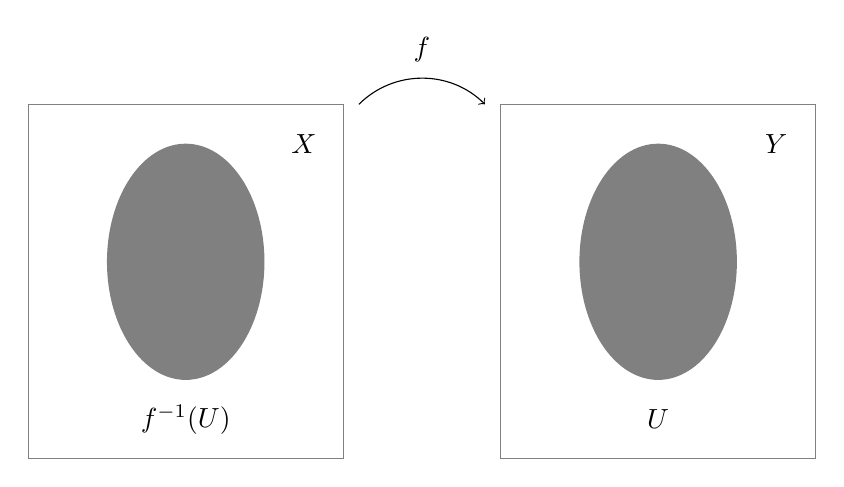
\begin{tikzpicture}
\draw[gray] (0,0) rectangle (4,4.5);
\node at (3.5,4) {$X$};

\draw[gray] (6,0) rectangle (10,4.5);
\node at (9.5,4) {$Y$};

\draw[->] (4.2,4.5) to [bend left=45] (5.8,4.5);
\node at (5,5.2) {$f$};

\fill[gray] (2,2.5) ellipse (1.0 and 1.5);
\node at (2,0.5) {$f^{-1}(U)$};

\fill[gray] (8,2.5) ellipse (1.0 and 1.5);
\node at (8,0.5) {$U$};
\end{tikzpicture}
\caption{Pre-image of a set}
\end{figure}

The definition of continuity in \cref{defn:continuity-topological-spaces} is a global one. 
Frequently it is desirable to define continuity locally:
\begin{quote}
$f\colon X\to Y$ is \emph{continuous} at $x_0\in X$ if, for every neighbourhood $U$ of $f(x_0)$, there exists a neighbourhood $V$ of $x_0$ such that $f(V)\subset U$. 
\end{quote}

When $X$ and $Y$ are metric spaces, the local and global definitions are equivalent. 
The following result relates the local and global definitions of continuity for topological spaces.

\begin{lemma}[Equivalent definitions for continuity]
Let $X$ and $Y$ be topological spaces. Then $f\colon X\to Y$ is continuous if and only if $f$ is continuous at every point of $X$. 
\end{lemma}

\begin{proof} \

\fbox{$\implies$} Suppose $f$ is continuous, let $x_0\in X$. 

Let $U$ be a neighbourhood of $f(x_0)$, then $U$ is open in $X$. By continuity of $f$, $f^{-1}(U)$ is open in $X$. Since
\begin{itemize}
\item $f^{-1}(U)$ is a neighbourhood of $x_0$, and
\item $f(f^{-1}(U))\subset U$,
\end{itemize}
it follows that $f$ is continuous at $x_0$.

\fbox{$\impliedby$} Suppose $f$ is continuous at every point of $X$.

Let $U$ be a open set in $Y$. By (local) continuity of $f$, every point $x\in f^{-1}(U)$ has a neighbourhood $V_x$ such that $f(V_x)\subset U$. Thus $V_x\subset f^{-1}(U)$. Since
\[f^{-1}(U)=\bigcup_{x}V_x,\]
$f^{-1}(U)$ is the union of open sets $V_x$, so $f^{-1}(U)$ is itself open. Hence $f$ is continuous.
\end{proof}

\begin{lemma}
Let $X$ and $Y$ be topological spaces; let $f\colon X\to Y$. Then the following are equivalent:
\begin{enumerate}[label=(\roman*)]
\item $f$ is continuous.
\item $f(\overline{A})\subset \overline{f(A)}$ for every $A\subset X$.
\item $f^{-1}(B)$ is closed in $X$ for every closed set $B$ of $Y$.
\item For each $x\in X$ and each neighbourhood $V$ of $f(x)$, there is a neighbourhood $U$ of $x$ such that $f(U)\subset V$.
\end{enumerate}
\end{lemma}

The next result states that continuous functions of continuous functions are continuous.

\begin{lemma}
Let $X$, $Y$ and $Z$ be topological spaces. If $f\colon X\to Y$ and $g\colon Y\to Z$ are continuous, then $h=g\circ f$ is continuous.
\end{lemma}

\begin{proof}
Let $U$ be open in $Z$. By continuity of $g$, we have that $g^{-1}(U)$ is open in $Y$. Note that
\[h^{-1}(U)=f^{-1}\brac{g^{-1}(U)}.\]
If $f$ is continuous, it follows that $h^{-1}(U)$ is open, so $h$ is continuous.
\end{proof}

\subsection{Homeomorphisms}
\begin{definition}
Let $X$ and $Y$ be topological spaces; let $f\colon X\to Y$ be a bijection. 
We say $f$ is a \vocab{homeomorphism}\index{homeomorphism} if both $f$ and its inverse $f^{-1}$ are continuous.
\end{definition}

\subsection{Constructing Continuous Functions}


\section{Metric Topology}
One of the most important and frequently used ways of imposing a topology on a set is to define the topology in terms of a metric on the set.

\begin{definition}

\end{definition}

\section{Quotient Topology}
\begin{definition}[Quotient map]
Let $X$ and $Y$ be topological spaces; let $p\colon X\to Y$ be a surjective map.
The map $p$ is said to be a \vocab{quotient map}\index{quotient map} if $U$ is open in $Y$ if and only if $p^{-1}(U)$ is open in $X$.
\end{definition}

\begin{definition}[Quotient topology]
If $X$ is a space and $A$ is a set and if $p\colon X\to A$ is a surjective map, then there exists exactly one topology $\mathcal{T}$ on $A$ relative to which $p$ is a quotient map; it is called the \vocab{quotient topology}\index{quotient topology} induced by $p$.
\end{definition}

\begin{lemma*}
The quotient topology $\mathcal{T}$ is a topology.
\end{lemma*}

\begin{definition}[Quotient space]
Let $X$ be a topological space, and let $X^*$ be a partition of $X$ into disjoint subsets whose union is $X$. Let $p\colon X\to X^*$ be the surjective map that carries each point of $X$ to the element of $X^*$ containing it. In the quotient topology induced by $p$, the space $X^*$ is called a \vocab{quotient space}\index{quotient space} of $X$.
\end{definition}